\section{Cross Sections}
\label{sec:cross_sections}

We introduce a new method of origami construction, using cross section disgrams.
Instead of beginning our construction from a 2-dimensional sheet of paper,
we consider a 1-dimensional cross section moving forwards in time.
A simple example is demonstrated in Figure~\ref{fig:strip_narrowing}.
\begin{figure}[htpb]
    \centering
    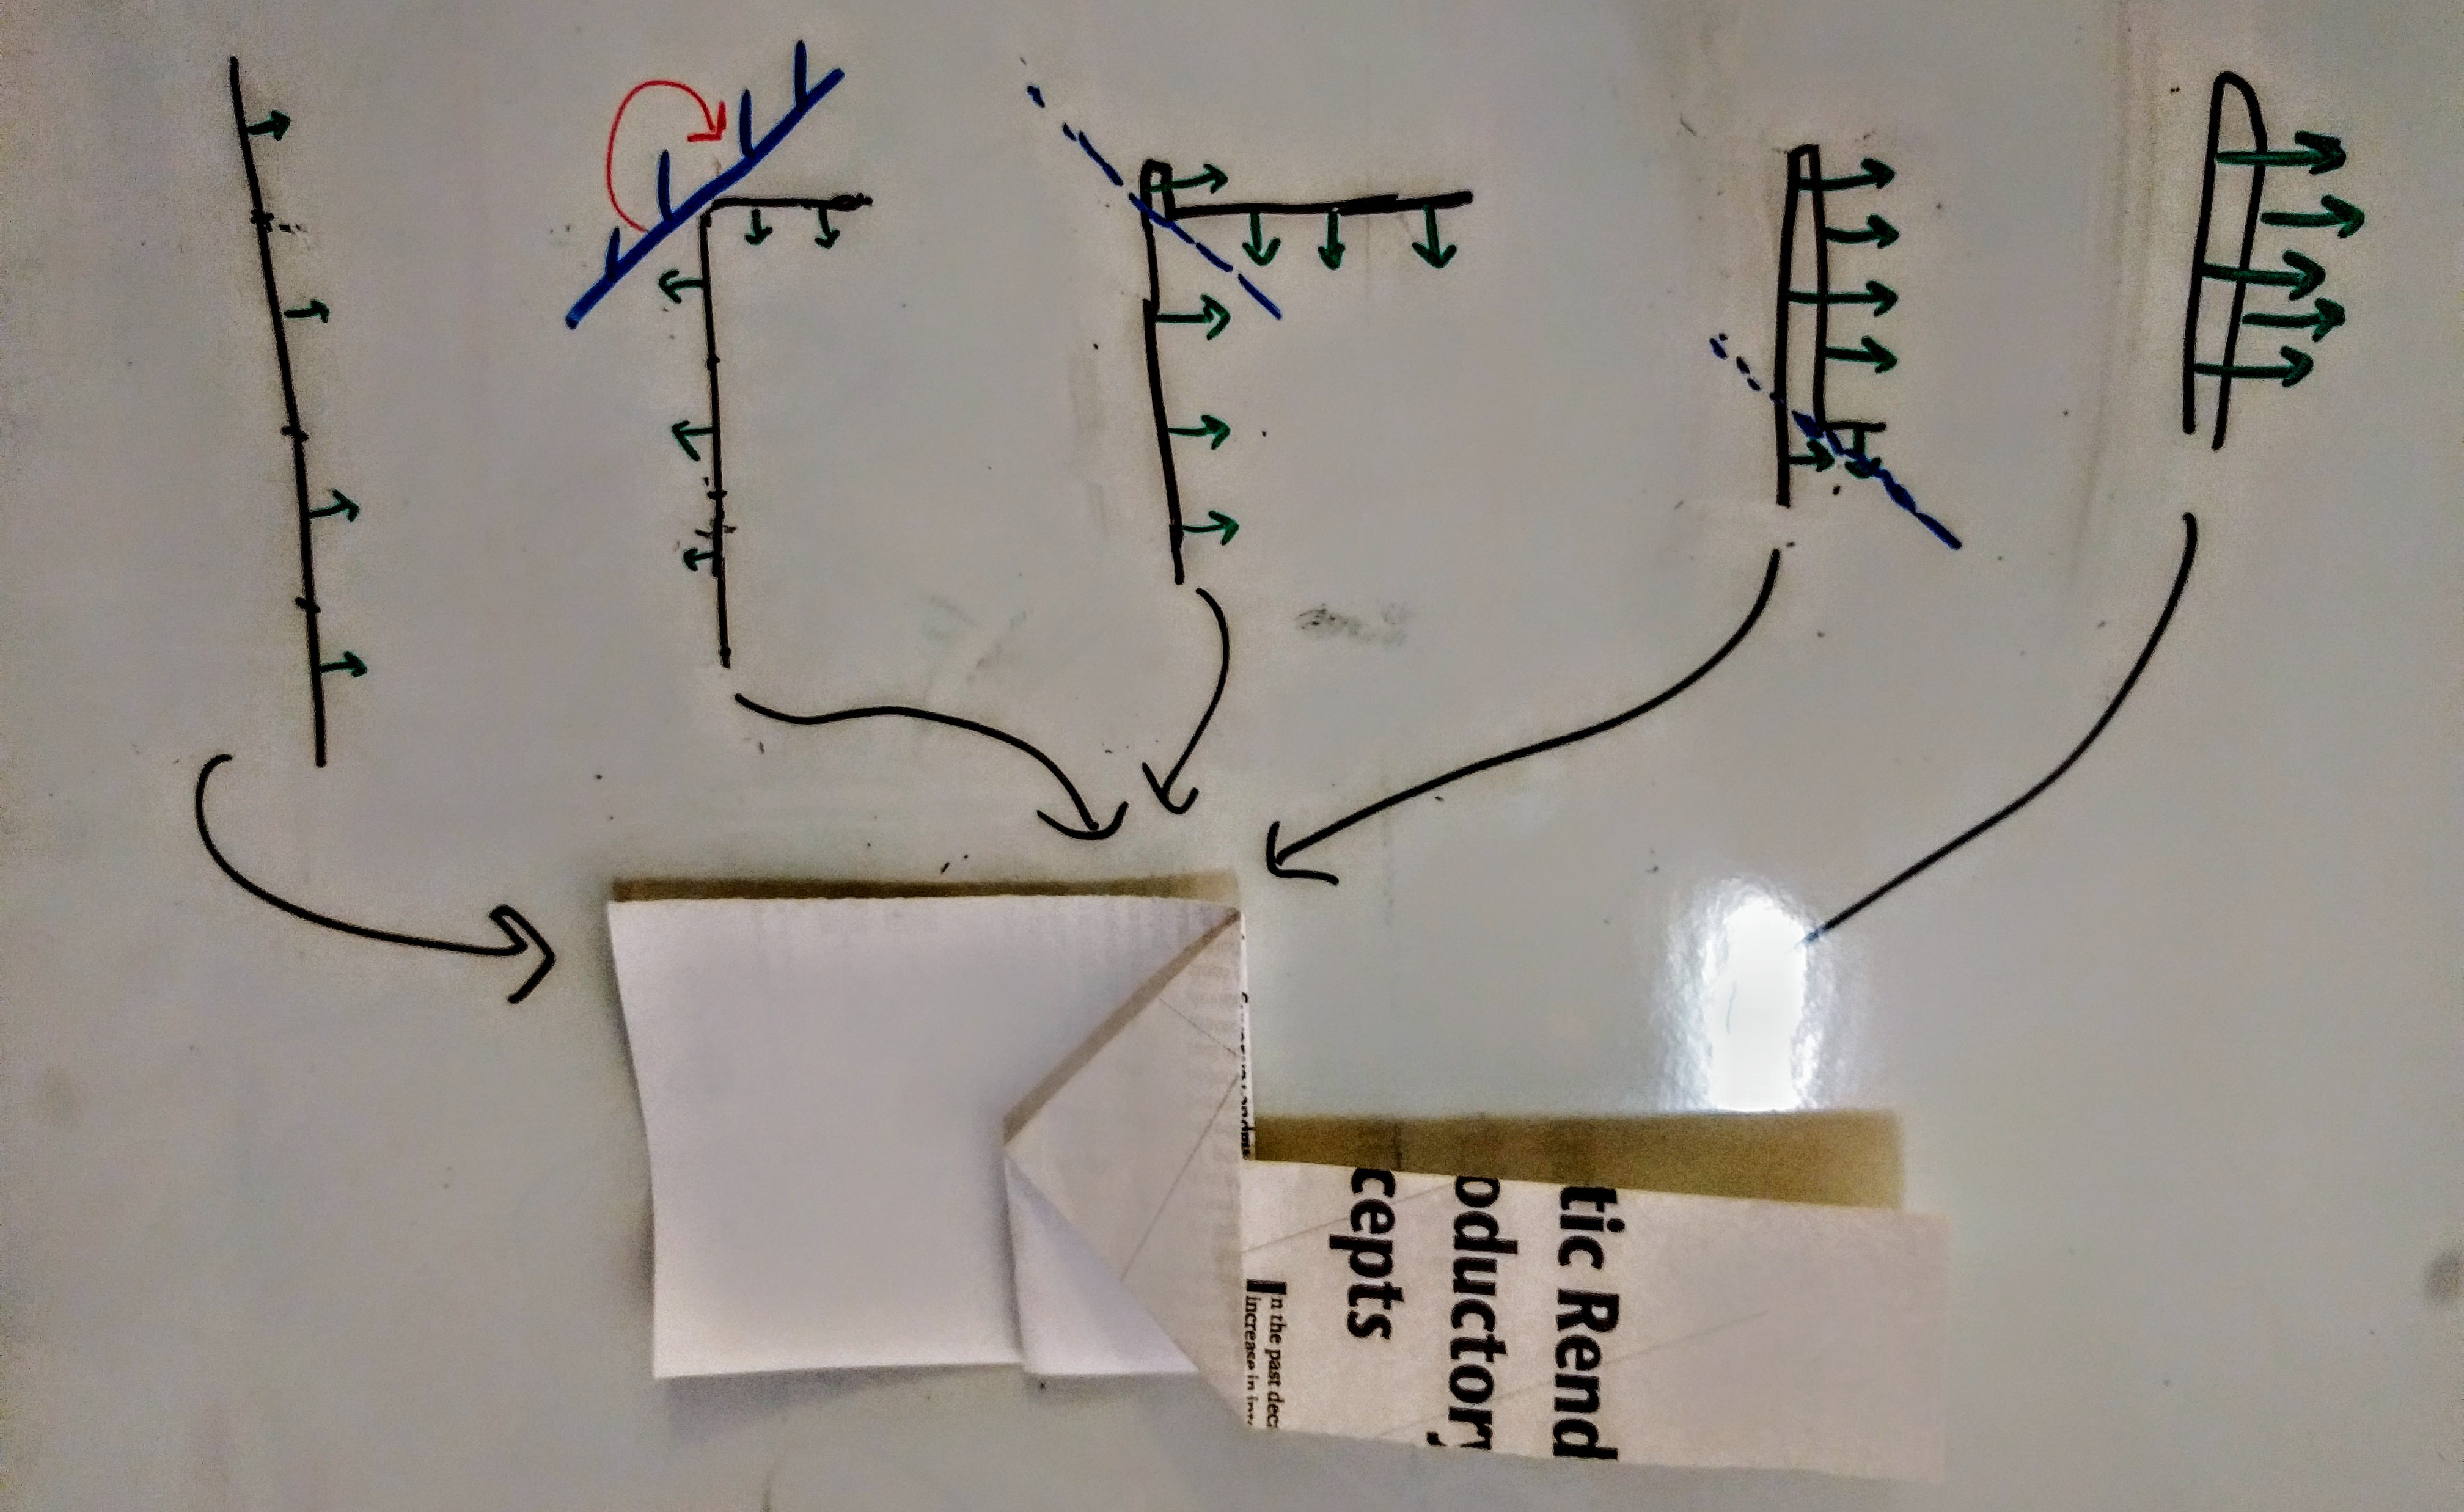
\includegraphics[width=0.8\linewidth]{figures/strip_narrowing.jpg}
    \caption{A strip narrowing gadget constructed from cross sections.}
    \label{fig:strip_narrowing}
\end{figure}

\subsection{Evolution}
\label{sec:evolution}

\subsubsection*{Segments and Velocities}
\label{sec:segments_and_velocities}
Divide the cross section into disjoint line segments, which share endpoints.

\subsubsection*{Evolution of Adjacent Segments}
\label{sec:evolution_of_adjacent_segments}
Each \emph{segment} has a direction associated with it (this should be perpendicular to the segment).
With the passage of time, segments may get shorter or longer.
This can result in a segment length becoming zero.

Note that time evolution is reversible.

\subsubsection*{Creation of New Segments}
\label{sec:creation_of_new_segments}
We may create a new segment at any point. Often the new segment has zero length.
In the event that an existing segment reaches length zero, we may modify \ldots

